\documentclass[12pt]{article}
\usepackage[margin=1in]{geometry}
\usepackage{amsmath}
\usepackage{booktabs}
\usepackage{graphicx}
\usepackage{tikz}
\usepackage{mathtools}  
\usepackage{xfrac}  
\usetikzlibrary{automata,positioning,arrows}
\newcommand\tab[1][1cm]{\hspace*{#1}}
\newcommand\n{\newline}
\newcommand\partiald[2]{
    \frac{\partial #1}{\partial #2}
}
\newcommand\ra{\rightarrow}

\begin{document}
CS7347 Test 1, Noah Gardner, 000843905\n

\begin{enumerate}
    \item \textbf{[Points 5]} Which of the following are correct for the given
          regular expression \verb/[\w.-]+@[\w.-]+/.
          \begin{enumerate}
              \item [a.] \verb/al.ice@yahoo.com/
              \item [b.] \verb/bob.alice-com/
              \item [c.] \verb/1.Abc@kennesaw.edu1/
              \item [d.] \verb/@ksu.edu/
              \item [e.] \verb/All of the above/
          \end{enumerate}

          \textbf{Answer:}
          \begin{description}
              \item \tab The grouping \verb/[\w.-]+/ matches the any character
                    in \verb/[a-zA-Z0-9_.-]/ between 1 and infinite number of
                    times. The \verb/@/ matches the \verb/@/ symbol literally.
                    $b$ is missing the symbol \verb/@/, and $d$ misses the first
                    grouping match. $e$ is incorrect since $b$ and $d$ are
                    incorrect. However, both $a$ and $c$ should match.

                    \textbf{Therefore, the answer is $a$ and $c$.}
          \end{description}

    \item \textbf{[Points 5]} Which of the followings are correct for the given
          regular expression \verb/^[^A-Z0-6]+/.
          \begin{enumerate}
              \item [a.] \verb/^abc 10/
              \item [b.] \verb/abc9/
              \item [c.] \verb/1 "Hello"/
              \item [d.] \verb/^abc9/
              \item [e.] \verb/None of the above/
          \end{enumerate}

          \textbf{Answer:}
          \begin{description}
              \item \tab The the first \verb/^/ token looks for a match at the
                    front of the line. The second \verb/^/ token tells us to
                    match any character not in \verb/[A-Z0-6]/ between 1 and
                    infinite number of times. $a$ is incorrect since it has a
                    space in the middle, however, the first half would match.
                    $b$ will match since \verb/abc9/ are not in \verb/[A-Z0-6]/.
                    $c$ is incorrect due to the space, also the first half of
                    the line does not match. Finally, $d$ will match since
                    \verb/^abc9/ are not in \verb/[A-Z0-6]/. $e$ is incorrect
                    since $b$ and $d$ match.

                    \textbf{Therefore, the answer is $b$ and $d$.}
          \end{description}

          \newpage
    \item \textbf{[Points 5]} Write down the differences of different activation
          functions, sigmoid, tanh, relu.

          \textbf{Answer:}
          \begin{description}
              \item \tab Activation functions are used in neural networks and
                    define the output of a node given it's inputs.

              \item \textbf{sigmoid}\n\tab The sigmoid function is a function
                    that outputs a value between 0 and 1. It is a non-linear
                    activation function and is widely used due to
                    differentiablity of the functon. However, the sigmoid
                    function may cause the neural network to get stuck in local
                    minima due to vanish gradient.
                    \begin{equation*}
                        y = 1/{1 + e^{-x}}
                    \end{equation*}

              \item \textbf{tanh}\n\tab The tanh function is a function that
                    outputs a value between -1 and 1. It is a non-linear
                    activation function similar to the sigmoid function. Due to
                    the larger range of the tanh activation function, it can
                    provide stronger gradients than the sigmoid function.
                    \begin{equation*}
                        y = (e^{x} - e^{-x})/(e^{x} + e^{-x})
                    \end{equation*}

              \item \textbf{relu}\n\tab The relu function is a function that
                    outputs a value between 0 and $\infty$. It is a linear
                    activation function, different from the sigmoid and tanh
                    functions. Additionally, the relu function does not have the
                    vanishing gradient problem, but instead has an opposite
                    problem called the \textit{exploding gradient} problem. The
                    exploding gradient problem can also be present in other
                    activation functions like tanh.
                    \begin{equation*}
                        y = max(0, x)
                    \end{equation*}
          \end{description}

          \newpage
    \item \textbf{[Points 5]} What is sequence labelling? How would you build
          your parts of speech baseline model?

          \textbf{Answer:}
          \begin{description}
              \item \tab Sequence labelling is a task in which a sequence of
                    words is labeled with a sequence of parts of speech.
                    Alternatively, sequence labelling can be used for name
                    entity recognition. To build a baseline model for parts of
                    speech tagging, you would require a training set of tagged
                    sentences as well as a model that can take sequential data
                    such as a sentence. Recurrent neural networks (RNN) work
                    well for this task.
          \end{description}

    \item \textbf{[Points 10]} What are name entities? What is entity
          recognition task? Give an NER example. Why is Name Entity Recognition
          (NER) a difficult task? Please describe with example, how window based
          NER classification can be performed to detect Person Name.

          \textbf{Answer:}
          \begin{description}
              \item \tab Name entities are entities that are recognized by a
                    computer program, similar to proper nouns. Name entities are
                    usually recognized by a computer program as a person,
                    location, organization, or other entity. NER is difficult
                    task because whether a word is a proper noun or not requires
                    a lot of context that typically can't be provided by just
                    the input sentence. It can also be hard to tell when the
                    name entity starts and ends. Therfore, a lot of training
                    data is required.

              \item \tab Window-based NER can be used to help provide context
                    for the word to be classified. For a given input sentence
                    and a given word $X_i$ we can train a softmax classifier.
                    For example, for a window size of 3, we have the following
                    input:
                    \begin{equation*}
                        X = [X_{i-2}*X_{i-1}*X_{i}*X_{i+1}*X_{i+2}]
                    \end{equation*}

                    To predict whether the input $X_i$ is a Person Name, we can
                    use a low value for \textit{not a Person Name} and a high
                    value for \textit{is a Person Name}. Then, given input $X$
                    and output ground-truth labels, we can use backpropagation
                    to train the model and make predictions.
          \end{description}

          \newpage
    \item \textbf{[Points 10]} Given the following equations:
          \begin{enumerate}
              \item $a = 3x + 4y$
              \item $b = 2x - 7y$
              \item $L = 2(a + b - z)$
          \end{enumerate}
          \begin{enumerate}
              \item Please draw computation graph (circuit diagram) for the
                    given equation above. \textbf{[Points 2]}
              \item Show forward pass values on the diagram, for the given
                    values of x=3, y=- 2 and z=1. \textbf{[Points 3]}

                    \textbf{Answer:}
                    \begin{figure}[h]
                        \centering
                        %% Machine generated by https://finsm.io
%% 2021-10-5-13:36:37
%% include in preamble:
%% \usepackage{tikz}
%% \usetikzlibrary{automata,positioning,arrows}
\begin{center}
    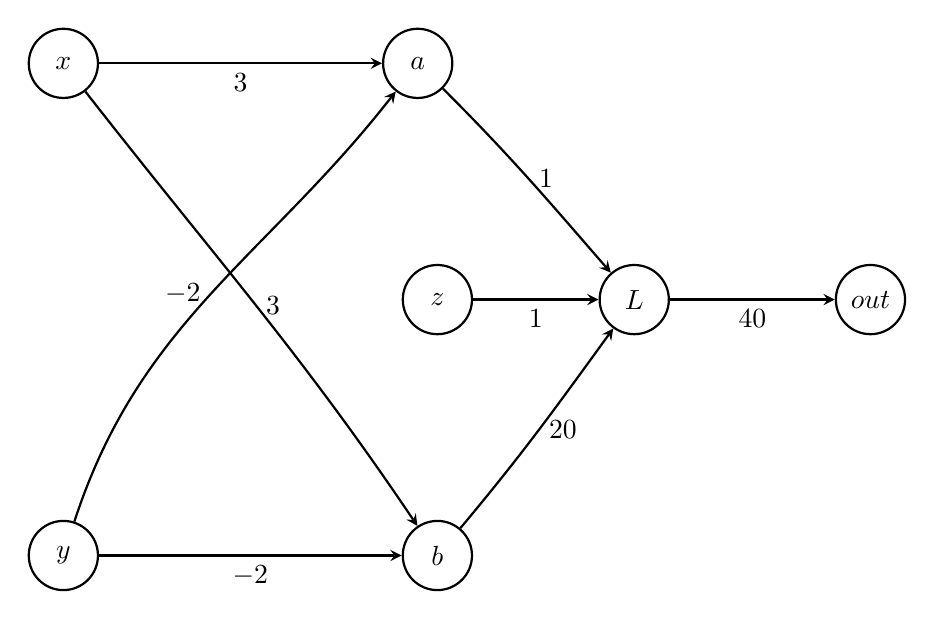
\begin{tikzpicture}[]
        \node[thick,state] at (-5,2) (85fb895c) {$x$};
        \node[thick,state] at (-5,-4.25) (47cbac90) {$y$};
        \node[thick,state] at (-0.5,2) (be9faf1d) {$a$};
        \node[thick,state] at (-0.25,-4.25) (86dd5d25) {$b$};
        \node[thick,state] at (2.25,-1) (b1778e2e) {$L$};
        \node[thick,state] at (5.25,-1) (a15a1e8d) {$out$};
        \node[thick,state] at (-0.25,-1) (6397e57c) {$z$};
        \path[->, thick, >=stealth]
        (85fb895c) edge [below,in = 180, out = 0] node {$3$} (be9faf1d)
        (85fb895c) edge [right,in = 124, out = -52] node {$3$} (86dd5d25)
        (47cbac90) edge [left,in = -128, out = 72] node {$-2$} (be9faf1d)
        (47cbac90) edge [below,in = 180, out = 0] node {$-2$} (86dd5d25)
        (be9faf1d) edge [right,in = 131, out = -45] node {$1$} (b1778e2e)
        (86dd5d25) edge [right,in = -126, out = 50] node {$20$} (b1778e2e)
        (b1778e2e) edge [below,in = 180, out = 0] node {$40$} (a15a1e8d)
        (6397e57c) edge [below,in = 180, out = 0] node {$1$} (b1778e2e)
        ;
    \end{tikzpicture}
\end{center}
                        \caption{Computation Graph - Forward Pass}
                    \end{figure}
                    \newpage
              \item Show a complete backpropagation circuit diagram with
                    corresponding gradient values. \textbf{[Points 5]}

                    \textbf{Answer:}\n\tab The nodes $x_2$, $y_2$, and
                    \textit{out} are used to show the backprop to the required
                    nodes due to limitations of the modelling software.
                    \begin{figure}[h]
                        \centering
                        %% Machine generated by https://finsm.io
%% 2021-10-5-13:34:34
%% include in preamble:
%% \usepackage{tikz}
%% \usetikzlibrary{automata,positioning,arrows}
\begin{center}
    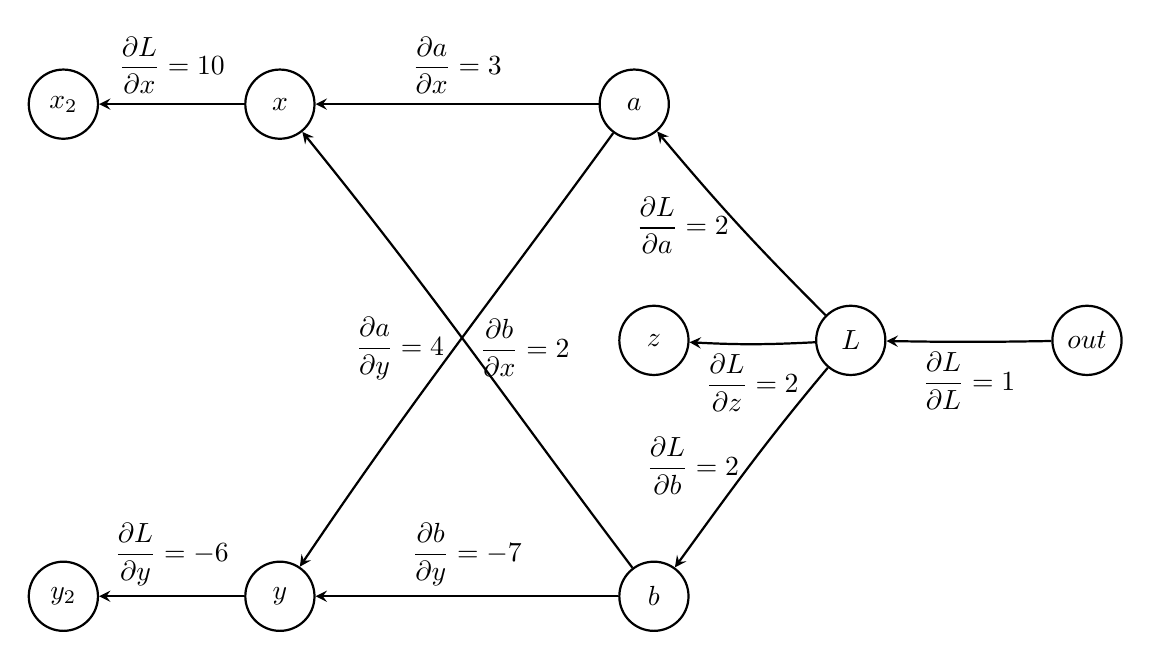
\begin{tikzpicture}[]
        \node[thick,state] at (-5,2) (9ee38db6) {$x$};
        \node[thick,state] at (-5,-4.25) (0c832477) {$y$};
        \node[thick,state] at (-0.5,2) (04d66450) {$a$};
        \node[thick,state] at (-0.25,-4.25) (301e0fe7) {$b$};
        \node[thick,state] at (2.25,-1) (f17d38c3) {$L$};
        \node[thick,state] at (5.25,-1) (a2dff366) {$out$};
        \node[thick,state] at (-0.25,-1) (2dfe7b55) {$z$};
        \node[thick,state] at (-7.75,2) (608cc445) {$x_2$};
        \node[thick,state] at (-7.75,-4.25) (49615258) {$y_2$};
        \path[->, thick, >=stealth]
        (9ee38db6) edge [above,in = 0, out = 180] node {$\dfrac{\partial L}{\partial x}=10$} (608cc445)
        (0c832477) edge [above,in = 0, out = 180] node {$\dfrac{\partial L}{\partial y}=-6$} (49615258)
        (04d66450) edge [above,in = 0, out = 180] node {$\dfrac{\partial a}{\partial x}=3$} (9ee38db6)
        (04d66450) edge [left,in = 56, out = -126] node {$\dfrac{\partial a}{\partial y}=4$} (0c832477)
        (301e0fe7) edge [right,in = -51, out = 127] node {$\dfrac{\partial b}{\partial x}=2$} (9ee38db6)
        (301e0fe7) edge [above,in = 0, out = 180] node {$\dfrac{\partial b}{\partial y}=-7$} (0c832477)
        (f17d38c3) edge [left,in = 54, out = -130] node {$\dfrac{\partial L}{\partial b}=2$} (301e0fe7)
        (f17d38c3) edge [left,in = -50, out = 135] node {$\dfrac{\partial L}{\partial a}=2$} (04d66450)
        (f17d38c3) edge [below,in = -3, out = -177] node {$\dfrac{\partial L}{\partial z}=2$} (2dfe7b55)
        (a2dff366) edge [below,in = -1, out = -179] node {$\dfrac{\partial L}{\partial L}=1$} (f17d38c3)
        ;
    \end{tikzpicture}
\end{center}
                        \caption{Computation Graph - Backpropagation}
                    \end{figure}

                    \begin{figure}[h]
                        \centering
                        {\renewcommand{\arraystretch}{1.5}
                            \begin{tabular}{|c|c|}
                                \hline
                                $\partiald{L}{L} = 1$ & $\partiald{a}{x} = 3$  \\
                                $\partiald{L}{a} = 2$ & $\partiald{a}{y} = 4$  \\
                                $\partiald{L}{b} = 2$ & $\partiald{b}{x} = 2$  \\
                                $\partiald{L}{z} = 2$ & $\partiald{b}{y} = -7$ \\
                                \hline
                            \end{tabular}}
                        {\renewcommand{\arraystretch}{1.5}
                            \begin{tabular}{|c|}
                                \hline
                                $\partiald{L}{x} = \partiald{L}{a}\partiald{a}{x} +
                                \partiald{L}{b}\partiald{b}{x} = 2*3 + 2*2 = 10$  \\
                                $\partiald{L}{y} = \partiald{L}{a}\partiald{a}{y} +
                                \partiald{L}{b}\partiald{b}{y} = 2*4 + 2*-7 = -6$ \\
                                \hline
                            \end{tabular}}
                        \caption{Partial Derivatives Calculations for Backpropagation}
                    \end{figure}
          \end{enumerate}
          \newpage
    \item \textbf{[Points 20]} You are given a large text corpus and a word2vec
          embeddings. You are building your Neural Language model (NN-language
          model) for your given corpus with two hidden layers. Please assume
          that you can choose your own configuration for these two layers (i.e.,
          number of neurons, etc.)
          \begin{enumerate}
              \item[a.] Please mention how would you build your NN-language
                  model using given word2vec embedding. Please show detailed
                  diagram and language model equations (forward pass only) for
                  each layer.
                  \textbf{[Points 10]}\n
                  \textbf{Answer:}

                  \tab Given word2vec embeddings, we can create a neural network
                  language model. This model will consist of an input layer,
                  which, on each timestep, will receive the word embedding of
                  context words (previous words in the sentence). The next layer
                  in the network is at least one hidden layer, although multiple
                  can be used.

                  The nodes in the input layer are connected to the
                  nodes in the output layer with a weight matrix. The nodes in
                  the hidden layer apply the activation function on the inputs
                  and output the results to the output layer. In the case of a
                  neural network language model, the output layer is a softmax
                  layer.

                  For our configuration, our NN-language model will consist of
                  an input layer, a hidden layer, and an output layer. The input
                  layer has a number of nodes equal to the size of the input
                  window for context words. We will use a window size of $3$.
                  For simplicity, the hidden layer will have $2$ nodes. Finally,
                  the output layer has a number of nodes equivalent to the
                  number of words in the vocabulary. Finally, our nodes will
                  have a sigmoid activation function. \textbf{See Figure
                      \ref{fig:nn_diagram} in the Appendix for more details.}

                  \begin{enumerate}
                      \item[1.] \textbf{First Layer (Input)}\n Given input
                          context words, output word embeddings of context words
                          from given embeddings. This will depend on the
                          training dataset but takes the form of a vector. We
                          apply a one-hot encoded vector to get our input
                          values.
                      \item[2.] \textbf{Second Layer (Hidden)}\n Word embeddings
                          of context words from first layer multiplied by the
                          weight $W_{ij}$ from input node $a_i$ to hidden node
                          $h_j$ plus the bias term $b_j$ as input to the
                          activation function.

                          \begin{equation*}
                              h_j = \sigma(W_{ij}a_i + b_j)
                          \end{equation*}

                      \item[3.] \textbf{Third Layer (Softmax)}\n $y_k$ is the
                          probability that the next word is the word $k$. The
                          output layer is a softmax layer, so the ouput from the
                          previous hidden layer is passed through a softmax
                          function to get the most probable word.

                          \begin{equation*}
                              \hat{y_k} = softmax(h)
                          \end{equation*}
                  \end{enumerate}
                  \newpage
              \item[b.] You decided to use your own word embedding instead of
                  word2vec. How would you design your NN-language model? Please
                  show details diagram and forward pass equation for your
                  language model. What are the parameters you need to train?
                  \textbf{[Points 10]}]\n
                  \textbf{Answer:}

                  \tab Since we will use our own word embedding, the first step
                  is to describe how it will work. Word embeddings allow us to
                  represent words in a vector space. We can use a
                  frequency-based approach to create our word embeddings. We
                  first count the number of occurences of each word in the
                  training set. Then, we can normalize the word embeddings by
                  using a standard normalization function, such as min-max
                  scaling.

                  After creating these embeddings, we can use the same
                  NN-language model as before. We have an input layer that takes
                  the word embeddings and feeds into a hidden layer. Then a
                  hidden layer feeds into our softmax output layer. Our proposed
                  embeddings may be less robust than word2vec embeddings,
                  however, they are simple to calculate. Other than frequencies,
                  there are no new parameters to train compared to the previous
                  model.
          \end{enumerate}
          \newpage
    \item \textbf{[Points 15]} Please build your character-gram (char-gram)
          language models for the given training set. Please assume that you
          experiment will only have the following characters – [a, b, c, d, f,
          h] that exists in the training set.

          \begin{tabular}{l}
              \textbf{Training set:} \\
              a a b c d b f          \\
              b c h a d f f a h      \\
              b b a a h c c h d d f  \\
              a b f f c c d f h      \\
              h h f f c a c d d d    \\
          \end{tabular}

          \begin{tabular}{l}
              \textbf{Test set:} \\
              a b c d f          \\
              a b b c c d        \\
          \end{tabular}

          \textbf{Task:}
          \begin{enumerate}
              \item[i.] Build char-unigram language model. \textbf{[Points 3]}
                  \n\textbf{Answer:}
                  \begin{figure}[h]
                      \centering
                      \begin{tabular}{|l|l|}
\hline
p(a) & $8/46$ \\
\hline
p(b) & $6/46$ \\
\hline
p(c) & $8/46$ \\
\hline
p(d) & $8/46$ \\
\hline
p(f) & $9/46$ \\
\hline
p(h) & $7/46$ \\
\hline
\end{tabular}
                      \caption{Char-unigram Model}
                  \end{figure}
                  \newpage
              \item[ii.] Build char-bigram language model. \textbf{[Points 3]}
                  \n\textbf{Answer:}
                  \begin{figure}[h]
                      \centering
                      \begin{tabular}{|l|l|}
\hline
p(a$|$a) & $2/8$ \\
\hline
p(a$|$b) & $1/6$ \\
\hline
p(a$|$begin) & $2/5$ \\
\hline
p(a$|$c) & $1/8$ \\
\hline
p(a$|$f) & $1/9$ \\
\hline
p(a$|$h) & $1/7$ \\
\hline
p(b$|$a) & $2/8$ \\
\hline
p(b$|$b) & $1/6$ \\
\hline
p(b$|$begin) & $2/5$ \\
\hline
p(b$|$d) & $1/8$ \\
\hline
p(c$|$a) & $1/8$ \\
\hline
p(c$|$b) & $2/6$ \\
\hline
p(c$|$c) & $2/8$ \\
\hline
p(c$|$f) & $2/9$ \\
\hline
p(c$|$h) & $1/7$ \\
\hline
p(d$|$a) & $1/8$ \\
\hline
p(d$|$c) & $3/8$ \\
\hline
p(d$|$d) & $3/8$ \\
\hline
p(d$|$h) & $1/7$ \\
\hline
p(end$|$d) & $1/8$ \\
\hline
p(end$|$f) & $2/9$ \\
\hline
p(end$|$h) & $2/7$ \\
\hline
p(f$|$b) & $2/6$ \\
\hline
p(f$|$d) & $3/8$ \\
\hline
p(f$|$f) & $3/9$ \\
\hline
p(f$|$h) & $1/7$ \\
\hline
p(h$|$a) & $2/8$ \\
\hline
p(h$|$begin) & $1/5$ \\
\hline
p(h$|$c) & $2/8$ \\
\hline
p(h$|$f) & $1/9$ \\
\hline
p(h$|$h) & $1/7$ \\
\hline
\end{tabular}
                      \caption{Char-bigram Model}
                  \end{figure}
                  \newpage
              \item[iii.] Compute joint probability for the given test set using
                  char-unigram model. \n\textbf{[Points 3]}
                  \n\textbf{Answer:}\n
                  \textbf{Unigram Joint Probabilities:}
                  \begin{description}
                      \item[a)] \verb/p(a b c d f)/ = \n
                          $p(a)*p(b)*p(c)*p(d)*p(f) =$ \n
                          $8/46*6/46*8/46*8/46*9/46 = 0.000134$\n\n
                          Therefore, the probability of the first sentence is \textbf{0.000134}.
                      \item[b)] \verb/p(a b b c c d)/ = \n
                          $p(a)*p(b)*p(b)*p(c)*p(c)*p(d) =$ \n
                          $8/46*6/46*6/46*8/46*8/46*8/46 = 0.000015$\n\n
                          Therefore, the probability of the second sentence is \textbf{0.000015}.
                  \end{description}

                  \newpage
              \item[iv.] Compute perplexity of your models (char-unigram,
                  char-bigram) and compare which model is better.
                  \textbf{[Points 6]}
                  \n\textbf{Answer:}\n

                  \tab Perplexity is defined as the inverse probability of the
                  test sentence normalized by the number of words (characaters,
                  in this case) in the sentence. The bigram model will have the
                  tokens \textit{begin} and \textit{end} inserted at the
                  beginning and end of each sentence to the probability of each
                  character as the beginning and end of the sentence. These
                  tokens will not count towards the total amount of words in the
                  sentence during the normalization step.

                  Since we have the joint probability using the unigram model,
                  calculate the probability of each sentence in the test set
                  with the bigram model:\n

                  \textbf{Bigram Joint Probabilities:}
                  \begin{description}
                      \item[a)] \verb/p(a b c d f)/ = \n
                          $p(a|begin)*p(b|a)*p(c|b)*p(d|c)*p(f|d)*p(end|f) =$ \n
                          $2/5*2/8*2/6*3/8*3/8*2/9 = 1/960 = 0.00104$\n\n
                          Therefore, the probability of the first sentence is \textbf{0.00104}.
                      \item[b)] \verb/p(a b b c c d)/ = \n
                          $p(a|begin)*p(b|a)*p(b|b)*p(c|b)*p(c|c)*p(d|c)*p(end|d) =$ \n
                          $2/5*2/8*1/6*2/6*2/8*3/8*1/8 = 1/15360 = 0.000065$\n\n
                          Therefore, the probability of the second sentence is \textbf{0.000065}.
                  \end{description}

                  \textbf{Unigram Perplexities:}
                  \begin{description}
                      \item[a)] $(0.000134)^{-1/5} = 5.95085$
                      \item[b)] $(0.000015)^{-1/6} = 6.36773$
                      \item[Average:] $(5.95085 + 6.36773)/2 =$ \textbf{6.15929}
                  \end{description}

                  \textbf{Bigram Perplexities:}
                  \begin{description}
                      \item[a)] $(0.00104)^{-1/5} = 3.94997$
                      \item[b)] $(0.000065)^{-1/6} = 4.9871$
                      \item[Average:] $(3.94997 + 4.9871)/2 =$ \textbf{4.46885}
                  \end{description}

                  The average perplexity of the bigram model is lower than the
                  unigram model. Because a lower perplexity indicates a better
                  performance, the bigram model is better than the unigram
                  model.
          \end{enumerate}

          \newpage
    \item \textbf{[Points 15]}  Assume that we are in an alien world and their
          languages are different and only contains the following vocabulary
              [\textit{delta, gamma, alpha, beta, sigma, derivative, summation}].
          Their parts-of-speech tags are given as [\textbf{A, B, C, D}].

          You are given a task to assign tags using Hidden Markov Model for the
          given test sentence. Given the following sentences as training
          examples:

          \begin{figure}[h]
              \centering
              \begin{tabular}{l|l}
                  \hline
                  Sentence 1: & \verb/delta gamma sigma summation/ \\
                  Tags:       & [\textbf{A, B, C, A}]   \\
                  \hline
                  Sentence 2: & \verb/alpha sigma beta derivative/ \\
                  Tags:       & [\textbf{A, C, D, A}]   \\
                  \hline
                  Sentence 3: & \verb/derivative gamma delta beta/ \\
                  Tags:       & [\textbf{A, B, B, D}]   \\
                  \hline
                  Sentence 4: & \verb/sigma summation beta alpha/ \\
                  Tags:       & [\textbf{C, B, C, D}]   \\
                  \hline
                  Sentence 5: & \verb/alpha beta sigma derivative/ \\
                  Tags:       & [\textbf{A, B, C, A}]   \\
              \end{tabular}
          \end{figure}

          \textbf{Test Sentence:} \verb/alpha gamma beta sigma/

          \begin{enumerate}
              \item[a.] Please calculate transition probabilities.
                  \textbf{[Points 3]}
                  \n\textbf{Answer:}\n\tab To calculate transition
                  probabilities, count the number of co-occurences for each tag
                  and divide by the total number of times the tag appears. We add
                  tags $S$ and $E$ to mark the beginning and end of the
                  sentence.
                  \begin{figure}[h]
                      \centering
                      \begin{tabular}{|l|l|l|l|l|l|l|}
                          \hline
                          \textbf{Tag} & A   & B   & C   & D   & E   & totals \\
                          \hline
                          \textbf{S}   & 4/5 & 1/5 & 0   & 0   & 0   & 5      \\
                          \textbf{A}   & 0   & 3/7 & 1/7 & 0   & 3/7 & 7      \\
                          \textbf{B}   & 0   & 1/5 & 3/5 & 1/5 & 0   & 5      \\
                          \textbf{C}   & 2/5 & 1/5 & 0   & 2/5 & 0   & 5      \\
                          \textbf{D}   & 1/3 & 0   & 0   & 0   & 2/3 & 3      \\
                          \hline
                      \end{tabular}
                      \caption{Transition Probabilities}
                  \end{figure}
                  \newpage
              \item[b.] Calculate emission probabilities. \textbf{[Points 3]}
                  \n\textbf{Answer:}\n\tab To calculate emission probabilities,
                  count each time a word is associated with each label, divided
                  by the total number of times a word is associated with that
                  label.
                  \begin{figure}[h]
                      \centering
                      \begin{tabular}{|l|l|l|l|l|}
                          \hline
                          \textbf{Word}       & A   & B   & C   & D   \\
                          \hline
                          \textbf{delta}      & 1/7 & 1/5 & 0   & 0   \\
                          \textbf{gamma}      & 0   & 2/5 & 0   & 0   \\
                          \textbf{alpha}      & 2/7 & 0   & 0   & 1/3 \\
                          \textbf{beta}       & 0   & 1/5 & 1/5 & 2/3 \\
                          \textbf{sigma}      & 0   & 0   & 4/5 & 0   \\
                          \textbf{derivative} & 3/7 & 0   & 0   & 0   \\
                          \textbf{summation}  & 1/7 & 1/5 & 0   & 0   \\
                          \textbf{totals}     & 7   & 5   & 5   & 3   \\
                          \hline
                      \end{tabular}
                      \caption{Emission Probabilities}
                  \end{figure}
                  \newpage
              \item[c.] How many  possible tag sequences (paths) can be
                  generated for the given test sentence? \textbf{[Points 3]}
                  \n\textbf{Answer:}\n\tab
                  \begin{description}
                      \item[Step 1.] \textbf{Add Emission Probabilities:} Using
                          the emission probabilities, we can create the following
                          tag sequence model.
                          \begin{figure}[h]
                              \centering
                              \includegraphics[width=0.65\textwidth]{assets/test1/emission1.png}
                          \end{figure}
                      \item[Step 2.] \textbf{Clean-up:} Remove all nodes with
                          emission probability of 0.
                          \begin{figure}[h]
                              \centering
                              \includegraphics[width=0.65\textwidth]{assets/test1/emission2.png}
                              \newpage
                          \end{figure}
                          \newpage
                      \item[Step 3.] \textbf{Add Transition Probabilities:}
                          Next, we add the transition probabilities.
                          \begin{figure}[h]
                              \centering
                              \includegraphics[width=0.65\textwidth]{assets/test1/transition1.png}
                          \end{figure}
                      \item[Step 4.] \textbf{Clean-up:} Remove all edges with
                          transition probability of 0 (excluding the only edge
                          leading to the node $E$). We then remove nodes that do
                          not have a valid sequence that will end in tag $E$.
                          \begin{figure}[h]
                              \centering
                              \includegraphics[width=0.65\textwidth]{assets/test1/transition2.png}
                          \end{figure}
                          \newpage
                      \item[Step 5.] \textbf{Padding:}

                          Since there are no transitions from a tag $C$ (the
                          only possible tag for \verb/sigma/ based on the
                          training set) to tag $E$, \textbf{there is only one
                              possible path at this step.} However, the transition
                          probability from the final to the end tag is 0. Since
                          this is unacceptable, we must remedy this in some way.
                          One approach is to pad the transition probability. We
                          can do so by adding $1$ to each cell in row $C$ and
                          recalculating the transition probabilities from tag
                          $C$.

                          \begin{figure}[h]
                              \centering
                              \begin{tabular}{|l|l|l|l|l|l|l|}
                                  \hline
                                  \textbf{Tag} & A            & B            & C            & D            & E            & totals     \\
                                  \hline
                                  \textbf{S}   & 4/5          & 1/5          & 0            & 0            & 0            & 5          \\
                                  \textbf{A}   & 0            & 3/7          & 1/7          & 0            & 3/7          & 7          \\
                                  \textbf{B}   & 0            & 1/5          & 3/5          & 1/5          & 0            & 5          \\
                                  \textbf{C}   & \textbf{3/9} & \textbf{2/9} & \textbf{1/9} & \textbf{3/9} & \textbf{1/9} & \textbf{9} \\
                                  \textbf{D}   & 1/3          & 0            & 0            & 0            & 2/3          & 3          \\
                                  \hline
                              \end{tabular}
                              \caption{Transition Probabilities \textbf{Modified}}
                          \end{figure}

                          \begin{figure}[h]
                              \centering
                              \includegraphics[width=0.65\textwidth]{assets/test1/transition3.png}
                          \end{figure}
                  \end{description}
                  \newpage
              \item[d.] Assign possible tags for the given test sentence
                  following maximum likelihood calculation. Please show details
                  likelihood calculation for all the optimized tag sequences.
                  \textbf{[Points 6]}
                  \n\textbf{Answer:}\n\tab With the transition probability
                  modified we can now calculate the maximum likelihood
                  probabilities. There is only one path, so there is only one
                  calculation.

                  \begin{equation*}
                      S\ra A\ra B\ra B\ra C\ra E =
                  \end{equation*}
                  \begin{equation*}
                      \frac{4}{5}*\frac{2}{7}*\frac{3}{7}*\frac{2}{5}*\frac{1}{5}*\frac{1}{5}*\frac{3}{5}*\frac{4}{5}*\frac{1}{9} = 0.00008359
                  \end{equation*}

                  Therefore, the assigned tags to the test sentence
                  \verb/alpha gamma beta sigma/ are \verb/[A, B, B, C]/.
                  However, this is somewhat unsatisfactory. To allow for more
                  possible tag sequences to be compared, the training set should
                  be expanded.
          \end{enumerate}

          \newpage
    \item \textbf{[Points 10]}  A restaurant chain wants to see whether
          customers like their foods or not. They hire you as an NLP scientist
          to do this task. You crawled their website, collect and annotate all
          the reviews. Your task is to conduct the experiment for this text
          data.

          \begin{enumerate}
              \item[a.] How many classes would you identify for this food review
                  and why? Please list down the class names as your preferences.
                  \textbf{[Points 2]}

                  \textbf{Answer:}
                  \begin{description}
                      \item \tab Since the chain would like to see whether
                            customers like (\textit{positive}) or dislike
                            (\textit{negative}), we can use the standard
                            approach for sentiment analysis, which utilizes
                            three classes: \textit{positive}, \textit{negative}
                            and \textit{neutral}. However, to allow for a
                            simpler model, we will use binary classification to
                            look for \textit{positive} and \textit{negative}
                            reviews and disregard \textit{neutral} reviews.
                  \end{description}
              \item[b.] You train two classifiers – (i) logistic
                  regression/softmax classifier, and (ii) a two-layer feed
                  forward neural network. Please mention differences between
                  these two classifiers. \textbf{[Points 3]}

                  \textbf{Answer:}
                  \begin{description}
                      \item \tab A logistic regression/softmax classifier is a
                            linear classifier that uses a logistic function to
                            make predictions. It is a binary classifier, which
                            means that it can only classify two classes, and
                            thus is suitable for this task. The logistic
                            function gives a probability for the class, then a
                            softmax function is used to normalize the output
                            to get the final class prediction.

                      \item \tab A two-layer feed forward neural network is a
                            feed forward neural network that has two hidden
                            layers. The neurons in each hidden layer of the
                            neural network have inputs, outputs, and a
                            differentiable activation function. The neurons are
                            also connected to the next layer through weights and
                            biases. The activation function allows the neuron to
                            take inputs and produce outputs. The output layer is
                            a fully connected layer with a softmax activation
                            function. Since the activation functions are
                            differentiable, we can use backpropagation in order
                            to train the model.
                  \end{description}
              \item[c.] Now you are deciding to pick only one classifier for the
                  deployment environment. How would you design your experimental
                  setup to evaluate these two classifiers? How would you decide
                  to pick which classifier for the deployment environment?
                  Please mention the details reason behind your decision.
                  \textbf{[Points 5]}

                  \textbf{Answer:}
                  \begin{description}
                      \item By using $k$-fold cross validation, we can evaluate
                            the average performance of each classifier with the
                            given input data set. It is common to use $k=10$,
                            but this will depend on the amount of available
                            data. With $10$-fold cross validation, first we
                            split the dataset into $10$ folds. We set aside $1$
                            fold for testing, and use the remaining $9$ folds
                            for training. We then train the classifier on the
                            training folds and test it on the testing fold. We
                            repeat this process $10$ times and save the final
                            evaluation score. At the end of training, we can
                            average the evaluation scores and compare the
                            performance of each model. Evaluation scores can
                            include precision, recall, and accuracy.
                  \end{description}
          \end{enumerate}
\end{enumerate}

\section{Appendix}
\begin{figure}[h]
    \centering
    \includegraphics[width=0.65\textwidth]{assets/test1/nn_diagram.jpg}
    \caption{NN-language Model}
    \label{fig:nn_diagram}
\end{figure}


\end{document}
